\chapter{Planteamiento del Problema}
\section{Descripción de la Realidad Problemática}

A nivel mundial, las tasas de presencia de cáncer de tiroides en personas varían de acuerdo con la edad, al género y al país. En el caso de Perú se tiene que por cada 100 000 mujeres existen 10.9 de casos de incidencia en este tipo de cáncer, y por cada 100 000 varones, se tiene un 3.6 de casos. Además de los casos de incidencia, la mortalidad también está presente y varía en varias partes del mundo. En Perú la mortalidad de pacientes mujeres con cáncer de tiroides es 1.7 por cada 100 000 personas, mientras que en los varones es de 0.77 casos cada 100 000 personas. \parencite{ws_oms2022cancert}

A continuación, se presentan dos gráficos que muestran los distintos índices de incidencia y mortalidad de cáncer de tiroides en mujeres, donde se puede resaltar la presencia de Perú en los rangos más altos de cada uno de estos. 

\begin{figure}[H]
	\begin{center}
		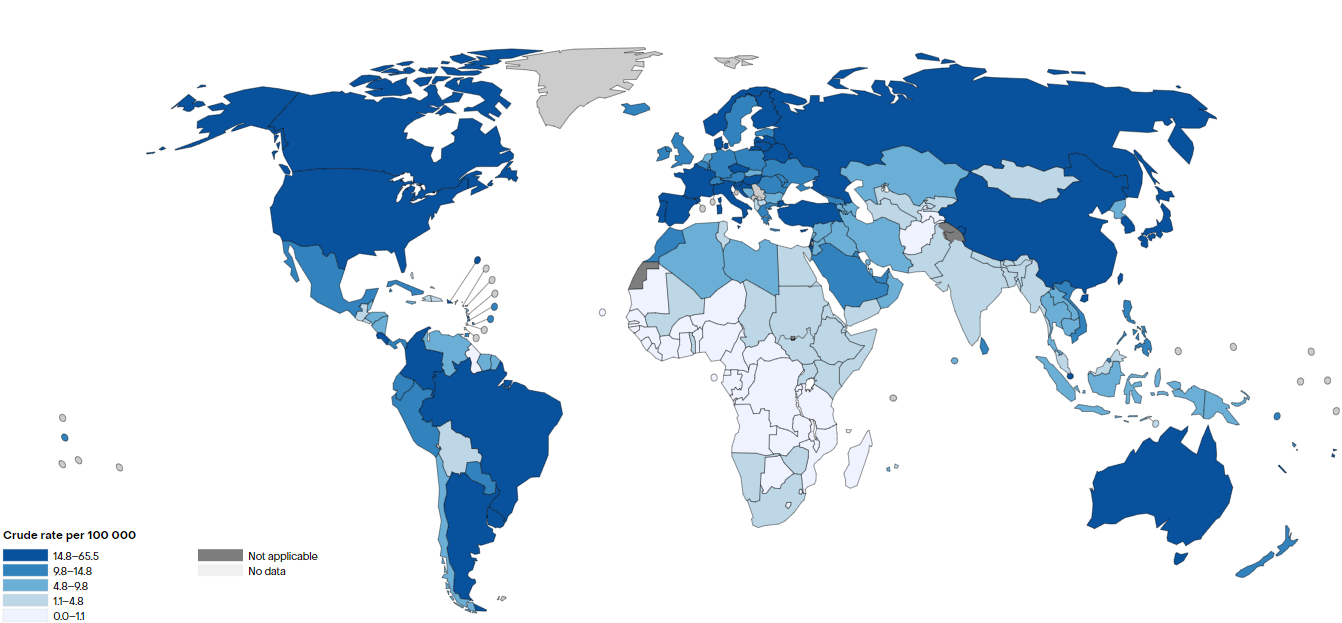
\includegraphics[width=1.00 \textwidth]{1/figures/tb_inc_ct_mujeres.png}
		\caption[Tasa bruta de incidencia de cáncer de tiroides en mujeres por 100 000 personas]{Tasa bruta de incidencia de cáncer de tiroides en mujeres por 100 000 personas. \\
		Fuente: \cite{ws_oms2022cancert}. \textit{Cancer Today}.}
		\label{1:fig}
	\end{center}
\end{figure}


\begin{figure}[H]
	\begin{center}
		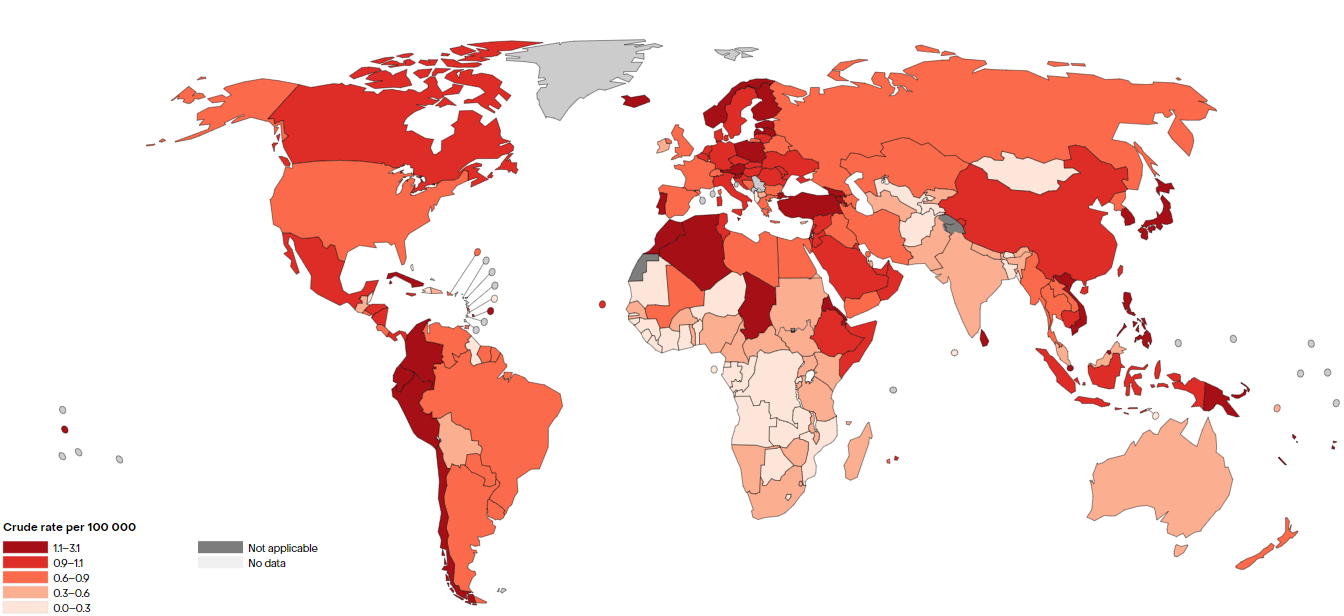
\includegraphics[width=1.00 \textwidth]{1/figures/tb_mor_ct_mujeres.png}
		\caption[Tasa bruta de mortalidad de cáncer de tiroides en mujeres por 100 000 personas]{Tasa bruta de mortalidad de cáncer de tiroides en mujeres por 100 000 personas. \\
		Fuente: \cite{ws_oms2022cancert}. \textit{Cancer Today}.}
		\label{1:fig2}
	\end{center}
\end{figure}

De igual forma, en el caso de los varones, el Perú también se encuentra entre los rangos más altos de incidencia y mortalidad. A continuación, se muestran sus respectivas gráficas.

\begin{figure}[H]
	\begin{center}
		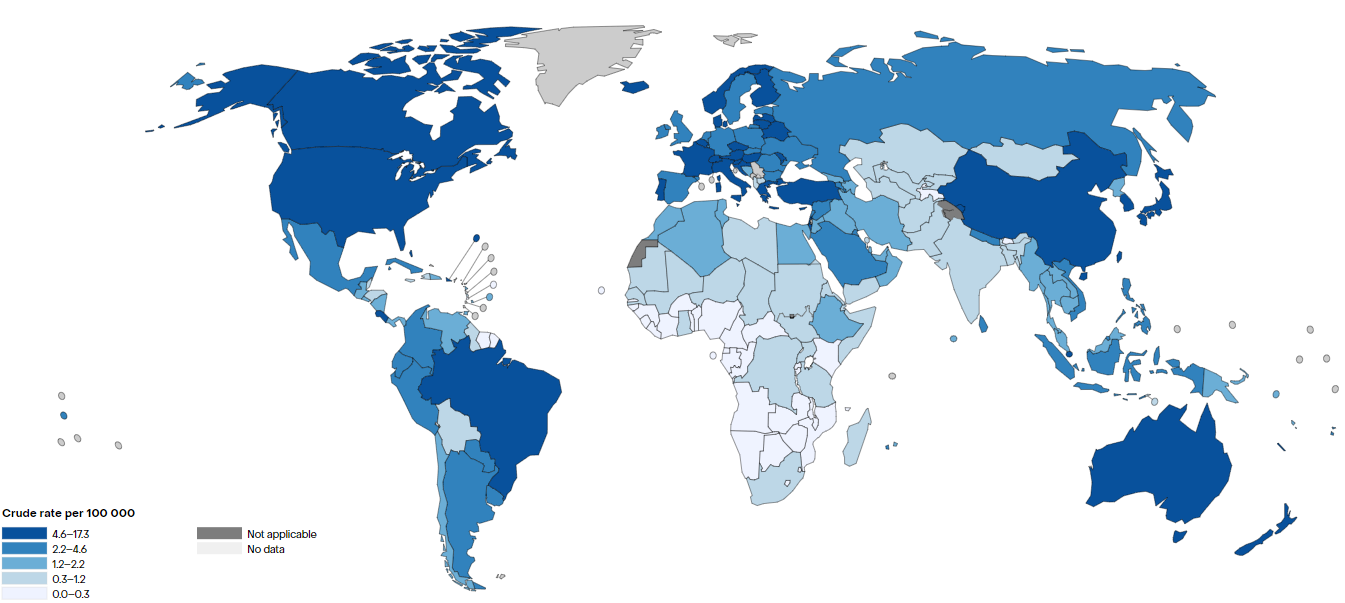
\includegraphics[width=1.00 \textwidth]{1/figures/tb_inc_ct_varones.png}
		\caption[Tasa bruta de incidencia de cáncer de tiroides en varones por 100 000 personas]{Tasa bruta de incidencia de cáncer de tiroides en varones por 100 000 personas. \\
		Fuente: \cite{ws_oms2022cancert}. \textit{Cancer Today}.}
		\label{1:fig3}
	\end{center}
\end{figure}

\begin{figure}[H]
	\begin{center}
		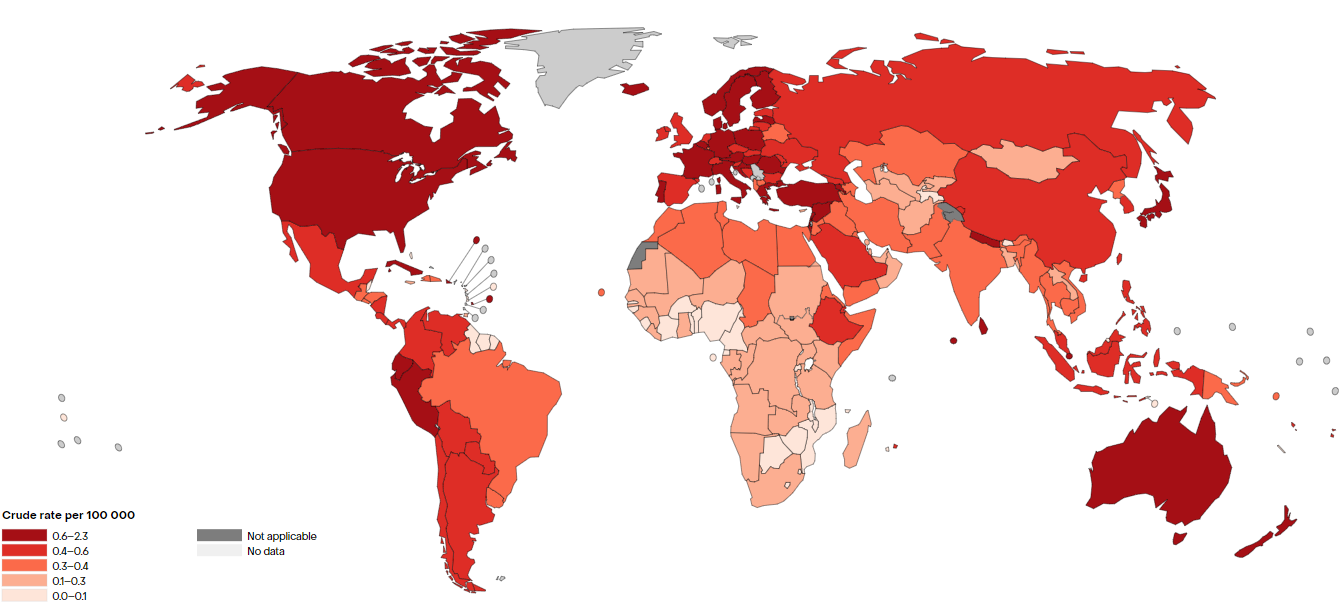
\includegraphics[width=1.00 \textwidth]{1/figures/tb_mor_ct_varones.png}
		\caption[Tasa bruta de mortalidad de cáncer de tiroides en varones por 100 000 personas]{Tasa bruta de mortalidad de cáncer de tiroides en varones por 100 000 personas. \\
		Fuente: \cite{ws_oms2022cancert}. \textit{Cancer Today}.}
		\label{1:fig4}
	\end{center}
\end{figure}

Con el siguiente gráfico que muestra los mismos índices distribuidos por género y regiones del mundo, es fácil notar la alta incidencia de este tipo de cáncer en las mujeres, siendo la región con mayor incidencia América del Norte, mientras que la de mayor mortalidad es Oceanía. La región de Latino América y el Caribe supera a Norte América en mortalidad, aunque se encuentra por debajo de Oceanía y Europa.

\begin{figure}[H]
	\begin{center}
		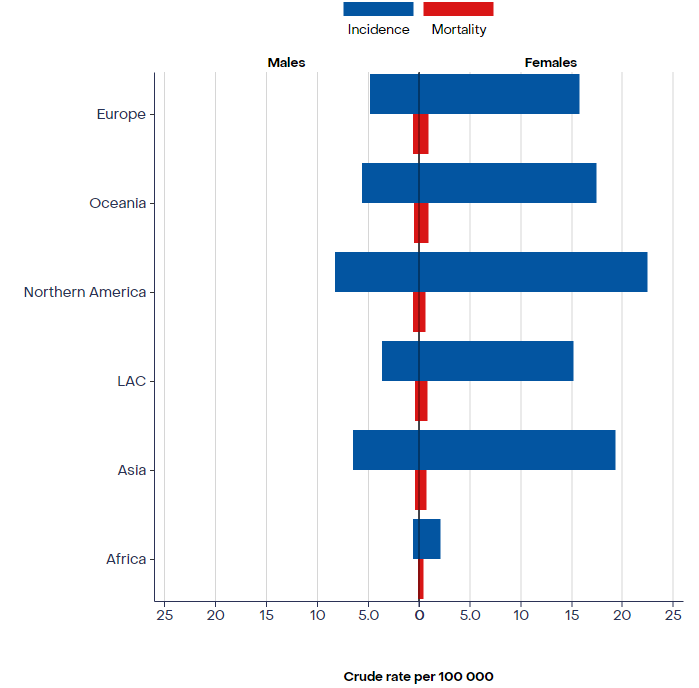
\includegraphics[width=0.60 \textwidth]{1/figures/tb_inc_mor_gen_y_reg.png}
		\caption[Tasa bruta de incidencia y mortalidad de cáncer de tiroides por género y región]{Tasa bruta de incidencia y mortalidad de cáncer de tiroides por género y región. \\
		Fuente: \cite{ws_oms2022cancert}. \textit{Cancer Today}.}
		\label{1:fig5}
	\end{center}
\end{figure}

Además, es importante mencionar que este aumento de incidencia a nivel global de cáncer de tiroides se debe a diversos factores relacionados a problemas de salud como la obesidad y a factores medioambientales como por ejemplo exposición al yodo \parencite{pr_kim2020geoinflu}. Sin embargo, otro factor es la poca disposición y capacidad de realizar un diagnóstico a tiempo de los nódulos tiroideos que, de forma general, cerca del 7\% al 15\% de los casos de llegan a ser cancerígenos \parencite{pr_haugen2016amethy}.

Para la detección temprana de este tipo de cáncer o desarrollo de tumores, depende en gran medida de la experiencia y la capacidad cognitiva de un experto en radiología, y muchos de estos se ven en la necesidad de utilizar no muy avanzados sistemas de pre-diagnóstico por computadora, mejor conocido como CAD por sus siglas en inglés \parencite{pr_zhu2021agendlframew}. Ante grandes limitaciones de sistemas CAD básicos, y aprovechando el extenso uso de la Inteligencia Artificial, el Deep Learning y sus algoritmos son capaces de incorporar mayor eficacia a dichos sistemas.

El Deep Learning ha sido usado ampliamente como herramienta para el procesamiento de imágenes médicas, no solo para detectar diferentes tipos de cáncer o nódulos como los relacionados a los pulmones, sino también para la retinopatía diabética y localización de feto en ecografías, e inclusive en la detección del COVID-19 \parencite{pr_bhatta2021medimage}. Además, el aumento de la calidad de imágenes de ultrasonido que se fue desarrollando en los últimos 30 años, aumentando cada vez más resolución de las imágenes y reduciendo el tiempo de adquisición, ha permitido una mejora en términos de detección de enfermedad; sin embargo, aún se requiere de un médico especializado y debidamente entrenado para lograr un realizar un correcto análisis de las imágenes, por ello se vio en la necesidad de encontrar métodos de clasificación automatizada, pero dichos métodos antiguos consumían bastante tiempo, gran poder computacional y poca capacidad de generalización de resultados, es así que en este contexto, apareció una novedosa arquitectura de Deep Learning que actualmente es usado en diferentes áreas el día de hoy: las Redes Neuronales Convolucionales o CNN, quitando en gran medida los problemas de las antigua técnicas \parencite{pr_signgh20203ddl}. Sin embargo, es importante mencionar que estos últimos años han ido apareciendo nuevas arquitecturas capaces incluso de superar a los ya altamente difundidos CNN. Y es que a pesar del dominio actual de estas redes, las arquitecturas basadas en Transformer han ido tomando cada vez más mayor importancia dentro del mundo de la Inteligencia Artificial, y esto incluye también el área de procesamiento de imágenes médicas gracias a los Vision Transformers o ViT, una versión de los Transformers originales orientados al procesamiento de imágenes.
 
El desarrollo de estas nuevas tecnologías basadas en distintos algoritmos de Inteligencia Artificial, ya sea en CNN, ViT o incluso ambos, podrían mejorar aún más los tiempos de pre-diagnóstico de nódulos tiroideos y, además, aumentar los porcentajes de aciertos de los especialistas en estas tareas de diagnóstico a través de un trabajo conjunto con estas tecnologías de alto potencial.



\section{Formulación del Problema}
Con el objetivo de formular los objetivos de esta investigación, se propusieron las siguientes preguntas.
\subsection{Problema General}
PG: \newcommand{\ProblemaGeneral}{
¿Es posible implementar un modelo de Deep Learning para el pre-diagnóstico de nódulos tiroideos a través de imágenes de ultrasonido?
}
\ProblemaGeneral
\subsection{Problemas Específicos}
\newcommand{\Pbone}{
¿Qué características del conjunto de datos a usar para entrenar y evaluar los modelos son ideales para obtener buenos resultados?
}
\newcommand{\Pbtwo}{
¿Qué técnicas de preprocesamiento se deberían aplicar a las imágenes de ultrasonido del conjunto de datos?
}
\newcommand{\Pbthree}{
¿De qué forma se puede evaluar el rendimiento de los modelos de Deep Learning en la clasificación de imágenes de ultrasonido?
}
\newcommand{\Pbfour}{
¿Qué arquitecturas de Deep Learning tienen el más alto desempeño en la clasificación de imágenes de ultrasonido de la tiroides?
}

\begin{itemize}
	\item PE1: {\Pbone}
	\item PE2: {\Pbtwo}
	\item PE3: {\Pbthree}
	\item PE4: {\Pbfour}
\end{itemize}

\section{Objetivos de la Investigación}
A continuación, se presentan el objetivo general y los objetivos específicos.
\subsection{Objetivo General}
OG: \newcommand{\ObjetivoGeneral}{
Diseñar un modelo de Deep Learning para el pre-diagnóstico de nódulos tiroideos a través de imágenes de ultrasonido.
}
\ObjetivoGeneral
\subsection{Objetivos Específicos}
\newcommand{\Objone}{
Determinar las características ideales del conjunto de datos a usar para entrenar y evaluar los modelos.
}
\newcommand{\Objtwo}{
Determinar las técnicas de preprocesamiento que se deben aplicar a las imágenes de ultrasonido del conjunto de datos.
}
\newcommand{\Objthree}{
Identificar las métricas de evaluación de rendimiento de los modelos de Deep Learning en la clasificación de imágenes de ultrasonido.
}
\newcommand{\Objfour}{
Determinar las arquitecturas de Deep Learning que tienen el más alto desempeño en la clasificación de imágenes de ultrasonido de la tiroides.
}

\begin{itemize}
	\item OE1: {\Objone}
	\item OE2: {\Objtwo}
	\item OE3: {\Objthree}
	\item OE4: {\Objfour}
\end{itemize}



\section{Justificación de la Investigación}

\subsection{Teórica}
Esta investigación plantea el desarrollo un modelo de Deep Learning capaz de pre-diagnosticar nódulos de la tiroides mediantes el uso de imágenes de ultrasonido. A través de este, se aborda el problema común de procesos de diagnóstico largos y, en gran porcentaje, inprecisos realizados por el personal especialista, ya que actualmente requiren de una extensa experiencia para lograr mejores resultados en este tipo de análisis de imágenes médicas. Además, la gran cantidad de investigaciones publicadas los últimos años sobre la Inteligencia Artificial han demostrado la alta capacidad de este tipo de tecnologías para desempeñarse en tareas como la detección, segmentación y clasificación enfocado en diversos campos. Específicamente el Deep Learning ha demostrado ser de las arquitecturas más preferidas para el procesamiento de imágenes, especialmente aquellas basadas en Redes Neuronales Convolucionales, los cuales, actualmente, están dominando las tareas relacionadas a imágenes por su alto desempeño. Sin embargo, estos últimos años, gracias al gran avance y divulgación de los modelos basados en Transformers, se ha visto el surgimiento de un nueva clase de arquitecturas que prometen mejorar el desempeño de los actuales modelos dominantes: los Vision Transformer (ViT). Siguiendo esta nueva tendencia, y obsservando el poco desarrollo actual de modelos ViT para el pre-diagnóstico de nódulos tiroideos, la investigación desarrollará modelos basados en ViT, además de los ya conocidos CNN.

\subsection{Práctica}
La investigación concluirá con una arquitectura de Inteligencia Artificial basada en Deep Learning de alto desempeño capaz de realizar el pre-diagnóstico de nódulos en la glándula de la tiroides, es decir, podrá determinar si un nódulo es benigno o maligno. Esto permitirá agilizar el proceso de diagnóstico realizado por las personas especialistas. Los beneficiarios finales serán todos los pacientes que pasen por este proceso de diagnóstico. Además, esta investigación evidenciará la capacidad de los modelos basados en arquitecturas de Deep Learning para realizar tareas de predicción (benigno o maligno) en base a imágenes de ultrasonido de la glándula de la tiroides.

\subsection{Metodológica}
El desarrollo de un modelo de Deep Learning para el pre-diagnóstico de nódulos tiroideos permitirá acelerar el proceso de diagnóstico a través de imágenes de ultrasonido, lo cual permitirá que los pacientes obtengan sus resultados de forma más rápida y eficiente, posteriormente, esto favorecerá a que el personal especialista determine los tratamientos adecuados lo más antes posible, llegando así a mejorar el bienestar de los pacientes, puesto que con un tratamiento a tiempo de los nódulos se puede evitar un posible cáncer en la glándula de la tiroides.

\section{Delimitación del Estudio}
A continuación, se presentará la delimitación espacial, temporal y conceptual.

\subsection{Espacial}
Debido a que la problemática y necesidad de diagnosticar a tiempo los nódulos tiroideos no es propio de una región o país, la data recopilada para realizar un correcto análisis de Inteligencia Artificial son basados en países extranjeros y de gran alcance como China, del cual se obtuvo el conjunto de datos de imágenes de ultrasonido. Los proyectos previos más afines al tema presentados en la investigación son desarrollados en diversos países extranjeros. 

\subsection{Temporal}
Los datos presentados en esta investigación sobre casos de incidencia y mortalidad de la tiroides son del año 2022. De igual forma, las imágenes de ultrasonido de glándulas de tiroides con presencia de nódulos que se usarán para entrenar y validar el modelo de clasificación son recopiladas del conjunto de datos de acceso libre TNCD publicada en el año 2022. Los antecedentes relacionados a esta investigación fueron publicados entre el 2019 y 2023.

\subsection{Conceptual}
La presente investigación se centrará en el desarrollo de un modelo de Deep Learning para realizar la clasificación de nódulos de la glándula de tiroides y así lograr determinar si es de carácter benigno o maligno. Esto se logrará a través del uso de diferentes arquitecturas como los basados en Redes Neuronales Convolucionales y los Vision Transformers. Estos modelos se desempeñarán en la tarea de análisis de imágenes médicas, específicamente, en imágenes de ultrasonido de la tiroides. Además, se usarán técnicas propias de la Inteligencia Artificial como la Transferencia de Aprendizaje y el Aumento de Datos para obtener mejores resultados. 
